\documentclass[1p]{elsarticle_modified}
%\bibliographystyle{elsarticle-num}

%\usepackage[colorlinks]{hyperref}
%\usepackage{abbrmath_seonhwa} %\Abb, \Ascr, \Acal ,\Abf, \Afrak
\usepackage{amsfonts}
\usepackage{amssymb}
\usepackage{amsmath}
\usepackage{amsthm}
\usepackage{scalefnt}
\usepackage{amsbsy}
\usepackage{kotex}
\usepackage{caption}
\usepackage{subfig}
\usepackage{color}
\usepackage{graphicx}
\usepackage{xcolor} %% white, black, red, green, blue, cyan, magenta, yellow
\usepackage{float}
\usepackage{setspace}
\usepackage{hyperref}

\usepackage{tikz}
\usetikzlibrary{arrows}

\usepackage{multirow}
\usepackage{array} % fixed length table
\usepackage{hhline}

%%%%%%%%%%%%%%%%%%%%%
\makeatletter
\renewcommand*\env@matrix[1][\arraystretch]{%
	\edef\arraystretch{#1}%
	\hskip -\arraycolsep
	\let\@ifnextchar\new@ifnextchar
	\array{*\c@MaxMatrixCols c}}
\makeatother %https://tex.stackexchange.com/questions/14071/how-can-i-increase-the-line-spacing-in-a-matrix
%%%%%%%%%%%%%%%

\usepackage[normalem]{ulem}

\newcommand{\msout}[1]{\ifmmode\text{\sout{\ensuremath{#1}}}\else\sout{#1}\fi}
%SOURCE: \msout is \stkout macro in https://tex.stackexchange.com/questions/20609/strikeout-in-math-mode

\newcommand{\cancel}[1]{
	\ifmmode
	{\color{red}\msout{#1}}
	\else
	{\color{red}\sout{#1}}
	\fi
}

\newcommand{\add}[1]{
	{\color{blue}\uwave{#1}}
}

\newcommand{\replace}[2]{
	\ifmmode
	{\color{red}\msout{#1}}{\color{blue}\uwave{#2}}
	\else
	{\color{red}\sout{#1}}{\color{blue}\uwave{#2}}
	\fi
}

\newcommand{\Sol}{\mathcal{S}} %segment
\newcommand{\D}{D} %diagram
\newcommand{\A}{\mathcal{A}} %arc


%%%%%%%%%%%%%%%%%%%%%%%%%%%%%5 test

\def\sl{\operatorname{\textup{SL}}(2,\Cbb)}
\def\psl{\operatorname{\textup{PSL}}(2,\Cbb)}
\def\quan{\mkern 1mu \triangleright \mkern 1mu}

\theoremstyle{definition}
\newtheorem{thm}{Theorem}[section]
\newtheorem{prop}[thm]{Proposition}
\newtheorem{lem}[thm]{Lemma}
\newtheorem{ques}[thm]{Question}
\newtheorem{cor}[thm]{Corollary}
\newtheorem{defn}[thm]{Definition}
\newtheorem{exam}[thm]{Example}
\newtheorem{rmk}[thm]{Remark}
\newtheorem{alg}[thm]{Algorithm}

\newcommand{\I}{\sqrt{-1}}
\begin{document}

%\begin{frontmatter}
%
%\title{Boundary parabolic representations of knots up to 8 crossings}
%
%%% Group authors per affiliation:
%\author{Yunhi Cho} 
%\address{Department of Mathematics, University of Seoul, Seoul, Korea}
%\ead{yhcho@uos.ac.kr}
%
%
%\author{Seonhwa Kim} %\fnref{s_kim}}
%\address{Center for Geometry and Physics, Institute for Basic Science, Pohang, 37673, Korea}
%\ead{ryeona17@ibs.re.kr}
%
%\author{Hyuk Kim}
%\address{Department of Mathematical Sciences, Seoul National University, Seoul 08826, Korea}
%\ead{hyukkim@snu.ac.kr}
%
%\author{Seokbeom Yoon}
%\address{Department of Mathematical Sciences, Seoul National University, Seoul, 08826,  Korea}
%\ead{sbyoon15@snu.ac.kr}
%
%\begin{abstract}
%We find all boundary parabolic representation of knots up to 8 crossings.
%
%\end{abstract}
%\begin{keyword}
%    \MSC[2010] 57M25 
%\end{keyword}
%
%\end{frontmatter}

%\linenumbers
%\tableofcontents
%
\newcommand\colored[1]{\textcolor{white}{\rule[-0.35ex]{0.8em}{1.4ex}}\kern-0.8em\color{red} #1}%
%\newcommand\colored[1]{\textcolor{white}{ #1}\kern-2.17ex	\textcolor{white}{ #1}\kern-1.81ex	\textcolor{white}{ #1}\kern-2.15ex\color{red}#1	}

{\Large $\underline{12a_{0865}~(K12a_{0865})}$}

\setlength{\tabcolsep}{10pt}
\renewcommand{\arraystretch}{1.6}
\vspace{1cm}\begin{tabular}{m{100pt}>{\centering\arraybackslash}m{274pt}}
\multirow{5}{120pt}{
	\centering
	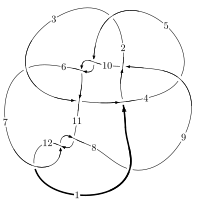
\includegraphics[width=112pt]{../../../GIT/diagram.site/Diagrams/png/1666_12a_0865.png}\\
\ \ \ A knot diagram\footnotemark}&
\allowdisplaybreaks
\textbf{Linearized knot diagam} \\
\cline{2-2}
 &
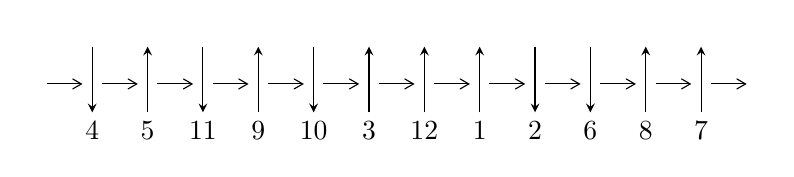
\begin{tikzpicture}[x=20pt, y=17pt]
	% nodes
	\node (C0) at (0, 0) {};
	\node (C1) at (1, 0) {};
	\node (C1U) at (1, +1) {};
	\node (C1D) at (1, -1) {4};

	\node (C2) at (2, 0) {};
	\node (C2U) at (2, +1) {};
	\node (C2D) at (2, -1) {5};

	\node (C3) at (3, 0) {};
	\node (C3U) at (3, +1) {};
	\node (C3D) at (3, -1) {11};

	\node (C4) at (4, 0) {};
	\node (C4U) at (4, +1) {};
	\node (C4D) at (4, -1) {9};

	\node (C5) at (5, 0) {};
	\node (C5U) at (5, +1) {};
	\node (C5D) at (5, -1) {10};

	\node (C6) at (6, 0) {};
	\node (C6U) at (6, +1) {};
	\node (C6D) at (6, -1) {3};

	\node (C7) at (7, 0) {};
	\node (C7U) at (7, +1) {};
	\node (C7D) at (7, -1) {12};

	\node (C8) at (8, 0) {};
	\node (C8U) at (8, +1) {};
	\node (C8D) at (8, -1) {1};

	\node (C9) at (9, 0) {};
	\node (C9U) at (9, +1) {};
	\node (C9D) at (9, -1) {2};

	\node (C10) at (10, 0) {};
	\node (C10U) at (10, +1) {};
	\node (C10D) at (10, -1) {6};

	\node (C11) at (11, 0) {};
	\node (C11U) at (11, +1) {};
	\node (C11D) at (11, -1) {8};

	\node (C12) at (12, 0) {};
	\node (C12U) at (12, +1) {};
	\node (C12D) at (12, -1) {7};
	\node (C13) at (13, 0) {};

	% arrows
	\draw[->,>={angle 60}]
	(C0) edge (C1) (C1) edge (C2) (C2) edge (C3) (C3) edge (C4) (C4) edge (C5) (C5) edge (C6) (C6) edge (C7) (C7) edge (C8) (C8) edge (C9) (C9) edge (C10) (C10) edge (C11) (C11) edge (C12) (C12) edge (C13) ;	\draw[->,>=stealth]
	(C1U) edge (C1D) (C2D) edge (C2U) (C3U) edge (C3D) (C4D) edge (C4U) (C5U) edge (C5D) (C6D) edge (C6U) (C7D) edge (C7U) (C8D) edge (C8U) (C9U) edge (C9D) (C10U) edge (C10D) (C11D) edge (C11U) (C12D) edge (C12U) ;
	\end{tikzpicture} \\
\hhline{~~} \\& 
\textbf{Solving Sequence} \\ \cline{2-2} 
 &
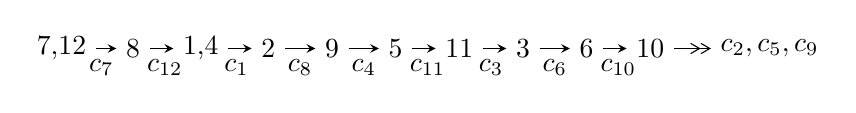
\begin{tikzpicture}[x=23pt, y=7pt]
	% node
	\node (A0) at (-1/8, 0) {7,12};
	\node (A1) at (1, 0) {8};
	\node (A2) at (33/16, 0) {1,4};
	\node (A3) at (25/8, 0) {2};
	\node (A4) at (33/8, 0) {9};
	\node (A5) at (41/8, 0) {5};
	\node (A6) at (49/8, 0) {11};
	\node (A7) at (57/8, 0) {3};
	\node (A8) at (65/8, 0) {6};
	\node (A9) at (73/8, 0) {10};
	\node (C1) at (1/2, -1) {$c_{7}$};
	\node (C2) at (3/2, -1) {$c_{12}$};
	\node (C3) at (21/8, -1) {$c_{1}$};
	\node (C4) at (29/8, -1) {$c_{8}$};
	\node (C5) at (37/8, -1) {$c_{4}$};
	\node (C6) at (45/8, -1) {$c_{11}$};
	\node (C7) at (53/8, -1) {$c_{3}$};
	\node (C8) at (61/8, -1) {$c_{6}$};
	\node (C9) at (69/8, -1) {$c_{10}$};
	\node (A10) at (11, 0) {$c_{2},c_{5},c_{9}$};

	% edge
	\draw[->,>=stealth]	
	(A0) edge (A1) (A1) edge (A2) (A2) edge (A3) (A3) edge (A4) (A4) edge (A5) (A5) edge (A6) (A6) edge (A7) (A7) edge (A8) (A8) edge (A9) ;
	\draw[->>,>={angle 60}]	
	(A9) edge (A10);
\end{tikzpicture} \\ 

\end{tabular} \\

\footnotetext{
The image of knot diagram is generated by the software ``\textbf{Draw programme}" developed by Andrew Bartholomew(\url{http://www.layer8.co.uk/maths/draw/index.htm\#Running-draw}), where we modified some parts for our purpose(\url{https://github.com/CATsTAILs/LinksPainter}).
}\phantom \\ \newline 
\centering \textbf{Ideals for irreducible components\footnotemark of $X_{\text{par}}$} 
 
\begin{align*}
I^u_{1}&=\langle 
5.19820\times10^{201} u^{139}+6.60058\times10^{201} u^{138}+\cdots+2.86650\times10^{201} b-1.70750\times10^{201},\\
\phantom{I^u_{1}}&\phantom{= \langle  }6.84846\times10^{202} u^{139}+1.27131\times10^{203} u^{138}+\cdots+2.86650\times10^{201} a-4.52189\times10^{203},\\
\phantom{I^u_{1}}&\phantom{= \langle  }u^{140}+2 u^{139}+\cdots-29 u-1\rangle \\
I^u_{2}&=\langle 
-17 u^{25}-137 u^{24}+\cdots+31 b-49,\;-127 u^{25}-274 u^{24}+\cdots+31 a-315,\;u^{26}+u^{25}+\cdots+6 u+1\rangle \\
\\
\end{align*}
\raggedright * 2 irreducible components of $\dim_{\mathbb{C}}=0$, with total 166 representations.\\
\footnotetext{All coefficients of polynomials are rational numbers. But the coefficients are sometimes approximated in decimal forms when there is not enough margin.}
\newpage
\renewcommand{\arraystretch}{1}
\centering \section*{I. $I^u_{1}= \langle 5.20\times10^{201} u^{139}+6.60\times10^{201} u^{138}+\cdots+2.87\times10^{201} b-1.71\times10^{201},\;6.85\times10^{202} u^{139}+1.27\times10^{203} u^{138}+\cdots+2.87\times10^{201} a-4.52\times10^{203},\;u^{140}+2 u^{139}+\cdots-29 u-1 \rangle$}
\flushleft \textbf{(i) Arc colorings}\\
\begin{tabular}{m{7pt} m{180pt} m{7pt} m{180pt} }
\flushright $a_{7}=$&$\begin{pmatrix}1\\0\end{pmatrix}$ \\
\flushright $a_{12}=$&$\begin{pmatrix}0\\u\end{pmatrix}$ \\
\flushright $a_{8}=$&$\begin{pmatrix}1\\- u^2\end{pmatrix}$ \\
\flushright $a_{1}=$&$\begin{pmatrix}u\\u\end{pmatrix}$ \\
\flushright $a_{4}=$&$\begin{pmatrix}-23.8914 u^{139}-44.3507 u^{138}+\cdots+3396.80 u+157.750\\-1.81343 u^{139}-2.30267 u^{138}+\cdots+38.5060 u+0.595675\end{pmatrix}$ \\
\flushright $a_{2}=$&$\begin{pmatrix}-4.24614 u^{139}-11.1656 u^{138}+\cdots+511.349 u+4.19872\\0.0697095 u^{139}-1.99479 u^{138}+\cdots-220.467 u-7.87942\end{pmatrix}$ \\
\flushright $a_{9}=$&$\begin{pmatrix}- u^4- u^2+1\\- u^4-2 u^2\end{pmatrix}$ \\
\flushright $a_{5}=$&$\begin{pmatrix}-27.0046 u^{139}-46.2135 u^{138}+\cdots+3518.44 u+162.574\\-1.23012 u^{139}+2.21877 u^{138}+\cdots-41.5813 u-2.31366\end{pmatrix}$ \\
\flushright $a_{11}=$&$\begin{pmatrix}- u\\u^3+u\end{pmatrix}$ \\
\flushright $a_{3}=$&$\begin{pmatrix}-25.2211 u^{139}-44.6624 u^{138}+\cdots+3446.08 u+160.211\\-0.652155 u^{139}+1.76471 u^{138}+\cdots-77.5282 u-4.21315\end{pmatrix}$ \\
\flushright $a_{6}=$&$\begin{pmatrix}13.6940 u^{139}+26.6243 u^{138}+\cdots-1236.53 u-28.6211\\2.72181 u^{139}+7.06780 u^{138}+\cdots-331.465 u-15.6455\end{pmatrix}$ \\
\flushright $a_{10}=$&$\begin{pmatrix}-0.00786984 u^{139}-1.16765 u^{138}+\cdots-309.091 u-43.0354\\-1.98484 u^{139}-8.29039 u^{138}+\cdots+454.057 u+21.0848\end{pmatrix}$\\&\end{tabular}
\flushleft \textbf{(ii) Obstruction class $= -1$}\\~\\
\flushleft \textbf{(iii) Cusp Shapes $= -6.89858 u^{139}-15.8047 u^{138}+\cdots+1204.83 u+62.7229$}\\~\\
\newpage\renewcommand{\arraystretch}{1}
\flushleft \textbf{(iv) u-Polynomials at the component}\newline \\
\begin{tabular}{m{50pt}|m{274pt}}
Crossings & \hspace{64pt}u-Polynomials at each crossing \\
\hline $$\begin{aligned}c_{1}\end{aligned}$$&$\begin{aligned}
&u^{140}+11 u^{139}+\cdots-24651 u-2513
\end{aligned}$\\
\hline $$\begin{aligned}c_{2}\end{aligned}$$&$\begin{aligned}
&u^{140}-9 u^{139}+\cdots+270 u+7
\end{aligned}$\\
\hline $$\begin{aligned}c_{3}\end{aligned}$$&$\begin{aligned}
&u^{140}-8 u^{138}+\cdots-94043 u+17197
\end{aligned}$\\
\hline $$\begin{aligned}c_{4}\end{aligned}$$&$\begin{aligned}
&u^{140}+3 u^{139}+\cdots+8798 u-3781
\end{aligned}$\\
\hline $$\begin{aligned}c_{5},c_{10}\end{aligned}$$&$\begin{aligned}
&u^{140}-50 u^{138}+\cdots-4 u-1
\end{aligned}$\\
\hline $$\begin{aligned}c_{6}\end{aligned}$$&$\begin{aligned}
&u^{140}+2 u^{139}+\cdots-20 u-1
\end{aligned}$\\
\hline $$\begin{aligned}c_{7},c_{11},c_{12}\end{aligned}$$&$\begin{aligned}
&u^{140}-2 u^{139}+\cdots+29 u-1
\end{aligned}$\\
\hline $$\begin{aligned}c_{8}\end{aligned}$$&$\begin{aligned}
&u^{140}+2 u^{139}+\cdots+1113371 u-44197
\end{aligned}$\\
\hline $$\begin{aligned}c_{9}\end{aligned}$$&$\begin{aligned}
&u^{140}-2 u^{139}+\cdots+71035 u-11231
\end{aligned}$\\
\hline
\end{tabular}\\~\\
\newpage\renewcommand{\arraystretch}{1}
\flushleft \textbf{(v) Riley Polynomials at the component}\newline \\
\begin{tabular}{m{50pt}|m{274pt}}
Crossings & \hspace{64pt}Riley Polynomials at each crossing \\
\hline $$\begin{aligned}c_{1}\end{aligned}$$&$\begin{aligned}
&y^{140}+y^{139}+\cdots-2719370831 y+6315169
\end{aligned}$\\
\hline $$\begin{aligned}c_{2}\end{aligned}$$&$\begin{aligned}
&y^{140}+15 y^{139}+\cdots-2382 y+49
\end{aligned}$\\
\hline $$\begin{aligned}c_{3}\end{aligned}$$&$\begin{aligned}
&y^{140}-16 y^{139}+\cdots-26838854679 y+295736809
\end{aligned}$\\
\hline $$\begin{aligned}c_{4}\end{aligned}$$&$\begin{aligned}
&y^{140}-25 y^{139}+\cdots-1468752308 y+14295961
\end{aligned}$\\
\hline $$\begin{aligned}c_{5},c_{10}\end{aligned}$$&$\begin{aligned}
&y^{140}-100 y^{139}+\cdots-192 y+1
\end{aligned}$\\
\hline $$\begin{aligned}c_{6}\end{aligned}$$&$\begin{aligned}
&y^{140}+8 y^{139}+\cdots+32 y+1
\end{aligned}$\\
\hline $$\begin{aligned}c_{7},c_{11},c_{12}\end{aligned}$$&$\begin{aligned}
&y^{140}+122 y^{139}+\cdots-197 y+1
\end{aligned}$\\
\hline $$\begin{aligned}c_{8}\end{aligned}$$&$\begin{aligned}
&y^{140}-44 y^{139}+\cdots-361041802395 y+1953374809
\end{aligned}$\\
\hline $$\begin{aligned}c_{9}\end{aligned}$$&$\begin{aligned}
&y^{140}-28 y^{139}+\cdots-7929328317 y+126135361
\end{aligned}$\\
\hline
\end{tabular}\\~\\
\newpage\flushleft \textbf{(vi) Complex Volumes and Cusp Shapes}
$$\begin{array}{c|c|c}  
\text{Solutions to }I^u_{1}& \I (\text{vol} + \sqrt{-1}CS) & \text{Cusp shape}\\
 \hline 
\begin{aligned}
u &= -0.699032 + 0.735483 I \\
a &= -0.002897 - 0.339529 I \\
b &= \phantom{-}0.213622 + 0.152636 I\end{aligned}
 & \phantom{-}0.77056 - 2.64531 I & \phantom{-0.000000 } 0 \\ \hline\begin{aligned}
u &= -0.699032 - 0.735483 I \\
a &= -0.002897 + 0.339529 I \\
b &= \phantom{-}0.213622 - 0.152636 I\end{aligned}
 & \phantom{-}0.77056 + 2.64531 I & \phantom{-0.000000 } 0 \\ \hline\begin{aligned}
u &= \phantom{-}0.544207 + 0.805924 I \\
a &= -0.489701 - 0.895906 I \\
b &= -0.438060 + 0.011080 I\end{aligned}
 & -4.10669 + 8.88255 I & \phantom{-0.000000 } 0 \\ \hline\begin{aligned}
u &= \phantom{-}0.544207 - 0.805924 I \\
a &= -0.489701 + 0.895906 I \\
b &= -0.438060 - 0.011080 I\end{aligned}
 & -4.10669 - 8.88255 I & \phantom{-0.000000 } 0 \\ \hline\begin{aligned}
u &= \phantom{-}0.394579 + 0.859613 I \\
a &= -1.131630 + 0.715654 I \\
b &= -0.079745 + 0.891189 I\end{aligned}
 & -0.29782 - 2.37813 I & \phantom{-0.000000 } 0 \\ \hline\begin{aligned}
u &= \phantom{-}0.394579 - 0.859613 I \\
a &= -1.131630 - 0.715654 I \\
b &= -0.079745 - 0.891189 I\end{aligned}
 & -0.29782 + 2.37813 I & \phantom{-0.000000 } 0 \\ \hline\begin{aligned}
u &= \phantom{-}0.472498 + 0.968616 I \\
a &= \phantom{-}0.829026 - 1.037290 I \\
b &= -0.219589 - 0.656120 I\end{aligned}
 & \phantom{-}1.70342 - 4.58350 I & \phantom{-0.000000 } 0 \\ \hline\begin{aligned}
u &= \phantom{-}0.472498 - 0.968616 I \\
a &= \phantom{-}0.829026 + 1.037290 I \\
b &= -0.219589 + 0.656120 I\end{aligned}
 & \phantom{-}1.70342 + 4.58350 I & \phantom{-0.000000 } 0 \\ \hline\begin{aligned}
u &= -0.460890 + 0.977356 I \\
a &= -0.88656 - 1.48895 I \\
b &= \phantom{-}0.362261 - 0.992992 I\end{aligned}
 & -3.34831 + 10.32660 I & \phantom{-0.000000 } 0 \\ \hline\begin{aligned}
u &= -0.460890 - 0.977356 I \\
a &= -0.88656 + 1.48895 I \\
b &= \phantom{-}0.362261 + 0.992992 I\end{aligned}
 & -3.34831 - 10.32660 I & \phantom{-0.000000 } 0\\
 \hline 
 \end{array}$$\newpage$$\begin{array}{c|c|c}  
\text{Solutions to }I^u_{1}& \I (\text{vol} + \sqrt{-1}CS) & \text{Cusp shape}\\
 \hline 
\begin{aligned}
u &= -0.286617 + 0.845325 I \\
a &= -1.022550 + 0.191229 I \\
b &= -0.283574 + 0.113795 I\end{aligned}
 & -0.20232 - 1.86529 I & \phantom{-0.000000 } 0 \\ \hline\begin{aligned}
u &= -0.286617 - 0.845325 I \\
a &= -1.022550 - 0.191229 I \\
b &= -0.283574 - 0.113795 I\end{aligned}
 & -0.20232 + 1.86529 I & \phantom{-0.000000 } 0 \\ \hline\begin{aligned}
u &= \phantom{-}0.798963 + 0.394167 I \\
a &= -0.0640261 + 0.0498232 I \\
b &= -0.630429 + 0.028242 I\end{aligned}
 & -2.77125 - 4.07901 I & \phantom{-0.000000 } 0 \\ \hline\begin{aligned}
u &= \phantom{-}0.798963 - 0.394167 I \\
a &= -0.0640261 - 0.0498232 I \\
b &= -0.630429 - 0.028242 I\end{aligned}
 & -2.77125 + 4.07901 I & \phantom{-0.000000 } 0 \\ \hline\begin{aligned}
u &= -0.853631 + 0.194477 I \\
a &= -0.1209890 + 0.0240797 I \\
b &= -0.471244 - 0.957436 I\end{aligned}
 & \phantom{-}4.00764 - 2.40019 I & \phantom{-0.000000 } 0 \\ \hline\begin{aligned}
u &= -0.853631 - 0.194477 I \\
a &= -0.1209890 - 0.0240797 I \\
b &= -0.471244 + 0.957436 I\end{aligned}
 & \phantom{-}4.00764 + 2.40019 I & \phantom{-0.000000 } 0 \\ \hline\begin{aligned}
u &= -0.806277 + 0.337217 I \\
a &= -0.323402 - 0.104556 I \\
b &= \phantom{-}0.326147 + 0.688530 I\end{aligned}
 & \phantom{-}1.29205 - 2.18437 I & \phantom{-0.000000 } 0 \\ \hline\begin{aligned}
u &= -0.806277 - 0.337217 I \\
a &= -0.323402 + 0.104556 I \\
b &= \phantom{-}0.326147 - 0.688530 I\end{aligned}
 & \phantom{-}1.29205 + 2.18437 I & \phantom{-0.000000 } 0 \\ \hline\begin{aligned}
u &= -0.234226 + 1.101490 I \\
a &= \phantom{-}1.30344 + 2.09572 I \\
b &= \phantom{-}0.30641 + 1.61658 I\end{aligned}
 & -4.83691 + 1.38716 I & \phantom{-0.000000 } 0 \\ \hline\begin{aligned}
u &= -0.234226 - 1.101490 I \\
a &= \phantom{-}1.30344 - 2.09572 I \\
b &= \phantom{-}0.30641 - 1.61658 I\end{aligned}
 & -4.83691 - 1.38716 I & \phantom{-0.000000 } 0\\
 \hline 
 \end{array}$$\newpage$$\begin{array}{c|c|c}  
\text{Solutions to }I^u_{1}& \I (\text{vol} + \sqrt{-1}CS) & \text{Cusp shape}\\
 \hline 
\begin{aligned}
u &= \phantom{-}0.835619 + 0.222340 I \\
a &= \phantom{-}0.1004540 - 0.0066237 I \\
b &= -0.82637 + 1.36466 I\end{aligned}
 & \phantom{-}4.00903 + 9.23441 I & \phantom{-0.000000 } 0 \\ \hline\begin{aligned}
u &= \phantom{-}0.835619 - 0.222340 I \\
a &= \phantom{-}0.1004540 + 0.0066237 I \\
b &= -0.82637 - 1.36466 I\end{aligned}
 & \phantom{-}4.00903 - 9.23441 I & \phantom{-0.000000 } 0 \\ \hline\begin{aligned}
u &= -0.836214 + 0.217940 I \\
a &= \phantom{-}0.0298363 - 0.0339143 I \\
b &= \phantom{-}1.10522 + 1.58007 I\end{aligned}
 & -1.0018 - 14.9566 I & \phantom{-0.000000 } 0 \\ \hline\begin{aligned}
u &= -0.836214 - 0.217940 I \\
a &= \phantom{-}0.0298363 + 0.0339143 I \\
b &= \phantom{-}1.10522 - 1.58007 I\end{aligned}
 & -1.0018 + 14.9566 I & \phantom{-0.000000 } 0 \\ \hline\begin{aligned}
u &= -0.512843 + 1.037880 I \\
a &= \phantom{-}0.448547 + 0.469658 I \\
b &= -0.060475 + 0.554886 I\end{aligned}
 & \phantom{-}1.44816 - 2.40172 I & \phantom{-0.000000 } 0 \\ \hline\begin{aligned}
u &= -0.512843 - 1.037880 I \\
a &= \phantom{-}0.448547 - 0.469658 I \\
b &= -0.060475 - 0.554886 I\end{aligned}
 & \phantom{-}1.44816 + 2.40172 I & \phantom{-0.000000 } 0 \\ \hline\begin{aligned}
u &= \phantom{-}0.793750 + 0.246725 I \\
a &= \phantom{-}0.293281 + 0.080782 I \\
b &= \phantom{-}0.43556 - 1.48959 I\end{aligned}
 & \phantom{-}1.69280 + 6.70388 I & \phantom{-0.000000 } 0 \\ \hline\begin{aligned}
u &= \phantom{-}0.793750 - 0.246725 I \\
a &= \phantom{-}0.293281 - 0.080782 I \\
b &= \phantom{-}0.43556 + 1.48959 I\end{aligned}
 & \phantom{-}1.69280 - 6.70388 I & \phantom{-0.000000 } 0 \\ \hline\begin{aligned}
u &= -0.824639\phantom{ +0.000000I} \\
a &= -0.567248\phantom{ +0.000000I} \\
b &= \phantom{-}1.18239\phantom{ +0.000000I}\end{aligned}
 & \phantom{-}0.488916\phantom{ +0.000000I} & \phantom{-0.000000 } 0 \\ \hline\begin{aligned}
u &= \phantom{-}0.154361 + 1.181950 I \\
a &= -1.68351 + 1.36233 I \\
b &= -0.540055 + 1.146340 I\end{aligned}
 & -1.56656 - 1.31155 I & \phantom{-0.000000 } 0\\
 \hline 
 \end{array}$$\newpage$$\begin{array}{c|c|c}  
\text{Solutions to }I^u_{1}& \I (\text{vol} + \sqrt{-1}CS) & \text{Cusp shape}\\
 \hline 
\begin{aligned}
u &= \phantom{-}0.154361 - 1.181950 I \\
a &= -1.68351 - 1.36233 I \\
b &= -0.540055 - 1.146340 I\end{aligned}
 & -1.56656 + 1.31155 I & \phantom{-0.000000 } 0 \\ \hline\begin{aligned}
u &= \phantom{-}0.793092\phantom{ +0.000000I} \\
a &= -0.0806651\phantom{ +0.000000I} \\
b &= \phantom{-}1.53427\phantom{ +0.000000I}\end{aligned}
 & -2.58349\phantom{ +0.000000I} & \phantom{-0.000000 } 0 \\ \hline\begin{aligned}
u &= \phantom{-}0.791372\phantom{ +0.000000I} \\
a &= \phantom{-}0.799386\phantom{ +0.000000I} \\
b &= \phantom{-}0.861709\phantom{ +0.000000I}\end{aligned}
 & \phantom{-}2.30047\phantom{ +0.000000I} & \phantom{-0.000000 } 0 \\ \hline\begin{aligned}
u &= -0.750566 + 0.146215 I \\
a &= -0.0957158 - 0.0484548 I \\
b &= -1.20575 - 1.93727 I\end{aligned}
 & -2.02859 - 5.11462 I & \phantom{-0.000000 } 0 \\ \hline\begin{aligned}
u &= -0.750566 - 0.146215 I \\
a &= -0.0957158 + 0.0484548 I \\
b &= -1.20575 + 1.93727 I\end{aligned}
 & -2.02859 + 5.11462 I & \phantom{-0.000000 } 0 \\ \hline\begin{aligned}
u &= \phantom{-}0.263724 + 1.213630 I \\
a &= -2.28924 + 1.40544 I \\
b &= -1.20765 + 1.17964 I\end{aligned}
 & -2.23381 - 2.33627 I & \phantom{-0.000000 } 0 \\ \hline\begin{aligned}
u &= \phantom{-}0.263724 - 1.213630 I \\
a &= -2.28924 - 1.40544 I \\
b &= -1.20765 - 1.17964 I\end{aligned}
 & -2.23381 + 2.33627 I & \phantom{-0.000000 } 0 \\ \hline\begin{aligned}
u &= \phantom{-}0.101179 + 1.246570 I \\
a &= \phantom{-}1.42493 - 1.52688 I \\
b &= \phantom{-}1.73158 - 1.63248 I\end{aligned}
 & -5.53848 - 4.43348 I & \phantom{-0.000000 } 0 \\ \hline\begin{aligned}
u &= \phantom{-}0.101179 - 1.246570 I \\
a &= \phantom{-}1.42493 + 1.52688 I \\
b &= \phantom{-}1.73158 + 1.63248 I\end{aligned}
 & -5.53848 + 4.43348 I & \phantom{-0.000000 } 0 \\ \hline\begin{aligned}
u &= -0.239253 + 1.231670 I \\
a &= -1.74160 + 0.07198 I \\
b &= -1.038660 - 0.033582 I\end{aligned}
 & -1.23220 - 2.64621 I & \phantom{-0.000000 } 0\\
 \hline 
 \end{array}$$\newpage$$\begin{array}{c|c|c}  
\text{Solutions to }I^u_{1}& \I (\text{vol} + \sqrt{-1}CS) & \text{Cusp shape}\\
 \hline 
\begin{aligned}
u &= -0.239253 - 1.231670 I \\
a &= -1.74160 - 0.07198 I \\
b &= -1.038660 + 0.033582 I\end{aligned}
 & -1.23220 + 2.64621 I & \phantom{-0.000000 } 0 \\ \hline\begin{aligned}
u &= -0.250859 + 1.242540 I \\
a &= \phantom{-}2.29923 + 1.40989 I \\
b &= \phantom{-}1.21683 + 2.45378 I\end{aligned}
 & -3.20135 + 1.99274 I & \phantom{-0.000000 } 0 \\ \hline\begin{aligned}
u &= -0.250859 - 1.242540 I \\
a &= \phantom{-}2.29923 - 1.40989 I \\
b &= \phantom{-}1.21683 - 2.45378 I\end{aligned}
 & -3.20135 - 1.99274 I & \phantom{-0.000000 } 0 \\ \hline\begin{aligned}
u &= -0.354369 + 1.218200 I \\
a &= \phantom{-}0.791897 - 0.893559 I \\
b &= \phantom{-}1.282500 + 0.117755 I\end{aligned}
 & -3.25883 - 4.26153 I & \phantom{-0.000000 } 0 \\ \hline\begin{aligned}
u &= -0.354369 - 1.218200 I \\
a &= \phantom{-}0.791897 + 0.893559 I \\
b &= \phantom{-}1.282500 - 0.117755 I\end{aligned}
 & -3.25883 + 4.26153 I & \phantom{-0.000000 } 0 \\ \hline\begin{aligned}
u &= \phantom{-}0.263563 + 1.244070 I \\
a &= -1.74414 + 0.50928 I \\
b &= -1.32904 + 1.54589 I\end{aligned}
 & \phantom{-}0.89939 + 1.62384 I & \phantom{-0.000000 } 0 \\ \hline\begin{aligned}
u &= \phantom{-}0.263563 - 1.244070 I \\
a &= -1.74414 - 0.50928 I \\
b &= -1.32904 - 1.54589 I\end{aligned}
 & \phantom{-}0.89939 - 1.62384 I & \phantom{-0.000000 } 0 \\ \hline\begin{aligned}
u &= \phantom{-}0.704979 + 0.164031 I \\
a &= -0.150435 + 0.275954 I \\
b &= \phantom{-}0.75076 - 1.65751 I\end{aligned}
 & \phantom{-}1.17772 + 4.48967 I & \phantom{-0.000000 } 0. - 7.53783 I \\ \hline\begin{aligned}
u &= \phantom{-}0.704979 - 0.164031 I \\
a &= -0.150435 - 0.275954 I \\
b &= \phantom{-}0.75076 + 1.65751 I\end{aligned}
 & \phantom{-}1.17772 - 4.48967 I & \phantom{-0.000000 -}0. + 7.53783 I \\ \hline\begin{aligned}
u &= -0.138523 + 1.273300 I \\
a &= \phantom{-}1.91958 + 1.67472 I \\
b &= \phantom{-}0.27945 + 1.45817 I\end{aligned}
 & -5.52155 + 3.54608 I & \phantom{-0.000000 } 0\\
 \hline 
 \end{array}$$\newpage$$\begin{array}{c|c|c}  
\text{Solutions to }I^u_{1}& \I (\text{vol} + \sqrt{-1}CS) & \text{Cusp shape}\\
 \hline 
\begin{aligned}
u &= -0.138523 - 1.273300 I \\
a &= \phantom{-}1.91958 - 1.67472 I \\
b &= \phantom{-}0.27945 - 1.45817 I\end{aligned}
 & -5.52155 - 3.54608 I & \phantom{-0.000000 } 0 \\ \hline\begin{aligned}
u &= \phantom{-}0.680138 + 0.223925 I \\
a &= -0.193380 + 0.683004 I \\
b &= -0.774622 + 1.149680 I\end{aligned}
 & -3.19836 + 6.87023 I & \phantom{-0.000000 } 0. - 7.99221 I \\ \hline\begin{aligned}
u &= \phantom{-}0.680138 - 0.223925 I \\
a &= -0.193380 - 0.683004 I \\
b &= -0.774622 - 1.149680 I\end{aligned}
 & -3.19836 - 6.87023 I & \phantom{-0.000000 -}0. + 7.99221 I \\ \hline\begin{aligned}
u &= \phantom{-}0.709719 + 0.068224 I \\
a &= -0.683746 - 0.317946 I \\
b &= \phantom{-}0.11986 - 1.99234 I\end{aligned}
 & \phantom{-}1.24243 + 5.87125 I & \phantom{-}6.34904 - 7.19748 I \\ \hline\begin{aligned}
u &= \phantom{-}0.709719 - 0.068224 I \\
a &= -0.683746 + 0.317946 I \\
b &= \phantom{-}0.11986 + 1.99234 I\end{aligned}
 & \phantom{-}1.24243 - 5.87125 I & \phantom{-}6.34904 + 7.19748 I \\ \hline\begin{aligned}
u &= -0.709889 + 0.062652 I \\
a &= -0.600356 + 0.023567 I \\
b &= -0.331801 + 0.869990 I\end{aligned}
 & \phantom{-}2.27965 - 0.78103 I & \phantom{-}5.12667 + 2.33382 I \\ \hline\begin{aligned}
u &= -0.709889 - 0.062652 I \\
a &= -0.600356 - 0.023567 I \\
b &= -0.331801 - 0.869990 I\end{aligned}
 & \phantom{-}2.27965 + 0.78103 I & \phantom{-}5.12667 - 2.33382 I \\ \hline\begin{aligned}
u &= \phantom{-}0.338264 + 1.242640 I \\
a &= \phantom{-}0.885981 + 0.992035 I \\
b &= \phantom{-}0.645640 + 0.882198 I\end{aligned}
 & -1.53639 + 4.07833 I & \phantom{-0.000000 } 0 \\ \hline\begin{aligned}
u &= \phantom{-}0.338264 - 1.242640 I \\
a &= \phantom{-}0.885981 - 0.992035 I \\
b &= \phantom{-}0.645640 - 0.882198 I\end{aligned}
 & -1.53639 - 4.07833 I & \phantom{-0.000000 } 0 \\ \hline\begin{aligned}
u &= -0.237859 + 1.267520 I \\
a &= \phantom{-}1.87506 + 0.52134 I \\
b &= \phantom{-}1.072570 + 0.110917 I\end{aligned}
 & -0.87635 - 1.45469 I & \phantom{-0.000000 } 0\\
 \hline 
 \end{array}$$\newpage$$\begin{array}{c|c|c}  
\text{Solutions to }I^u_{1}& \I (\text{vol} + \sqrt{-1}CS) & \text{Cusp shape}\\
 \hline 
\begin{aligned}
u &= -0.237859 - 1.267520 I \\
a &= \phantom{-}1.87506 - 0.52134 I \\
b &= \phantom{-}1.072570 - 0.110917 I\end{aligned}
 & -0.87635 + 1.45469 I & \phantom{-0.000000 } 0 \\ \hline\begin{aligned}
u &= -0.153130 + 1.286400 I \\
a &= -2.33191 - 0.81105 I \\
b &= -2.28428 - 1.09051 I\end{aligned}
 & -2.59239 - 0.40513 I & \phantom{-0.000000 } 0 \\ \hline\begin{aligned}
u &= -0.153130 - 1.286400 I \\
a &= -2.33191 + 0.81105 I \\
b &= -2.28428 + 1.09051 I\end{aligned}
 & -2.59239 + 0.40513 I & \phantom{-0.000000 } 0 \\ \hline\begin{aligned}
u &= \phantom{-}0.702759 + 0.035024 I \\
a &= \phantom{-}0.853019 + 0.137797 I \\
b &= -0.55503 - 1.35140 I\end{aligned}
 & \phantom{-}4.60287 + 1.87168 I & \phantom{-}11.89122 - 4.10578 I \\ \hline\begin{aligned}
u &= \phantom{-}0.702759 - 0.035024 I \\
a &= \phantom{-}0.853019 - 0.137797 I \\
b &= -0.55503 + 1.35140 I\end{aligned}
 & \phantom{-}4.60287 - 1.87168 I & \phantom{-}11.89122 + 4.10578 I \\ \hline\begin{aligned}
u &= \phantom{-}0.335754 + 0.602836 I \\
a &= \phantom{-}0.93091 - 1.29214 I \\
b &= \phantom{-}0.421732 - 0.159334 I\end{aligned}
 & -4.69130 - 3.41875 I & -4.42625 + 2.23362 I \\ \hline\begin{aligned}
u &= \phantom{-}0.335754 - 0.602836 I \\
a &= \phantom{-}0.93091 + 1.29214 I \\
b &= \phantom{-}0.421732 + 0.159334 I\end{aligned}
 & -4.69130 + 3.41875 I & -4.42625 - 2.23362 I \\ \hline\begin{aligned}
u &= -0.678583 + 0.049366 I \\
a &= -0.957749 + 0.458206 I \\
b &= \phantom{-}0.36880 - 2.25617 I\end{aligned}
 & \phantom{-}0.45229 - 5.35060 I & \phantom{-}7.25971 + 5.20115 I \\ \hline\begin{aligned}
u &= -0.678583 - 0.049366 I \\
a &= -0.957749 - 0.458206 I \\
b &= \phantom{-}0.36880 + 2.25617 I\end{aligned}
 & \phantom{-}0.45229 + 5.35060 I & \phantom{-}7.25971 - 5.20115 I \\ \hline\begin{aligned}
u &= \phantom{-}0.282654 + 1.290250 I \\
a &= \phantom{-}1.09719 - 1.34918 I \\
b &= -0.056532 - 0.990814 I\end{aligned}
 & \phantom{-}0.47298 + 5.43679 I & \phantom{-0.000000 } 0\\
 \hline 
 \end{array}$$\newpage$$\begin{array}{c|c|c}  
\text{Solutions to }I^u_{1}& \I (\text{vol} + \sqrt{-1}CS) & \text{Cusp shape}\\
 \hline 
\begin{aligned}
u &= \phantom{-}0.282654 - 1.290250 I \\
a &= \phantom{-}1.09719 + 1.34918 I \\
b &= -0.056532 + 0.990814 I\end{aligned}
 & \phantom{-}0.47298 - 5.43679 I & \phantom{-0.000000 } 0 \\ \hline\begin{aligned}
u &= \phantom{-}0.216260 + 1.312170 I \\
a &= \phantom{-}0.402189 + 0.478964 I \\
b &= \phantom{-}0.851919 - 0.831079 I\end{aligned}
 & -7.97931 + 2.80431 I & \phantom{-0.000000 } 0 \\ \hline\begin{aligned}
u &= \phantom{-}0.216260 - 1.312170 I \\
a &= \phantom{-}0.402189 - 0.478964 I \\
b &= \phantom{-}0.851919 + 0.831079 I\end{aligned}
 & -7.97931 - 2.80431 I & \phantom{-0.000000 } 0 \\ \hline\begin{aligned}
u &= -0.255683 + 1.305510 I \\
a &= -0.90800 - 1.66526 I \\
b &= -0.70433 - 2.40393 I\end{aligned}
 & -1.28242 - 4.99790 I & \phantom{-0.000000 } 0 \\ \hline\begin{aligned}
u &= -0.255683 - 1.305510 I \\
a &= -0.90800 + 1.66526 I \\
b &= -0.70433 + 2.40393 I\end{aligned}
 & -1.28242 + 4.99790 I & \phantom{-0.000000 } 0 \\ \hline\begin{aligned}
u &= -0.295633 + 1.297610 I \\
a &= \phantom{-}0.644611 + 1.000810 I \\
b &= \phantom{-}0.45480 + 1.38839 I\end{aligned}
 & -1.96637 - 4.43266 I & \phantom{-0.000000 } 0 \\ \hline\begin{aligned}
u &= -0.295633 - 1.297610 I \\
a &= \phantom{-}0.644611 - 1.000810 I \\
b &= \phantom{-}0.45480 - 1.38839 I\end{aligned}
 & -1.96637 + 4.43266 I & \phantom{-0.000000 } 0 \\ \hline\begin{aligned}
u &= -0.270539 + 1.306760 I \\
a &= -1.98197 - 2.10546 I \\
b &= -0.25403 - 1.98172 I\end{aligned}
 & -3.79851 - 8.78428 I & \phantom{-0.000000 } 0 \\ \hline\begin{aligned}
u &= -0.270539 - 1.306760 I \\
a &= -1.98197 + 2.10546 I \\
b &= -0.25403 + 1.98172 I\end{aligned}
 & -3.79851 + 8.78428 I & \phantom{-0.000000 } 0 \\ \hline\begin{aligned}
u &= -0.616335 + 0.237274 I \\
a &= -0.050993 + 1.088220 I \\
b &= -0.87278 - 1.49764 I\end{aligned}
 & -2.54122 - 5.60876 I & -1.84378 + 7.59056 I\\
 \hline 
 \end{array}$$\newpage$$\begin{array}{c|c|c}  
\text{Solutions to }I^u_{1}& \I (\text{vol} + \sqrt{-1}CS) & \text{Cusp shape}\\
 \hline 
\begin{aligned}
u &= -0.616335 - 0.237274 I \\
a &= -0.050993 - 1.088220 I \\
b &= -0.87278 + 1.49764 I\end{aligned}
 & -2.54122 + 5.60876 I & -1.84378 - 7.59056 I \\ \hline\begin{aligned}
u &= \phantom{-}0.288865 + 1.311520 I \\
a &= \phantom{-}2.04975 - 1.85069 I \\
b &= \phantom{-}1.44642 - 2.60044 I\end{aligned}
 & -3.08162 + 9.48378 I & \phantom{-0.000000 } 0 \\ \hline\begin{aligned}
u &= \phantom{-}0.288865 - 1.311520 I \\
a &= \phantom{-}2.04975 + 1.85069 I \\
b &= \phantom{-}1.44642 + 2.60044 I\end{aligned}
 & -3.08162 - 9.48378 I & \phantom{-0.000000 } 0 \\ \hline\begin{aligned}
u &= \phantom{-}0.196363 + 1.336460 I \\
a &= \phantom{-}2.42702 + 0.15394 I \\
b &= \phantom{-}2.07468 - 0.64978 I\end{aligned}
 & -8.11323 + 3.27890 I & \phantom{-0.000000 } 0 \\ \hline\begin{aligned}
u &= \phantom{-}0.196363 - 1.336460 I \\
a &= \phantom{-}2.42702 - 0.15394 I \\
b &= \phantom{-}2.07468 + 0.64978 I\end{aligned}
 & -8.11323 - 3.27890 I & \phantom{-0.000000 } 0 \\ \hline\begin{aligned}
u &= -0.647650 + 0.036056 I \\
a &= \phantom{-}1.364760 - 0.168535 I \\
b &= \phantom{-}0.230064 - 1.253090 I\end{aligned}
 & \phantom{-}2.93048 - 1.72674 I & \phantom{-}7.21258 + 2.95499 I \\ \hline\begin{aligned}
u &= -0.647650 - 0.036056 I \\
a &= \phantom{-}1.364760 + 0.168535 I \\
b &= \phantom{-}0.230064 + 1.253090 I\end{aligned}
 & \phantom{-}2.93048 + 1.72674 I & \phantom{-}7.21258 - 2.95499 I \\ \hline\begin{aligned}
u &= -0.415644 + 0.496287 I \\
a &= \phantom{-}1.06763 + 1.02386 I \\
b &= -0.884039 + 0.741752 I\end{aligned}
 & -3.46790 + 2.34643 I & -3.04341 - 0.92950 I \\ \hline\begin{aligned}
u &= -0.415644 - 0.496287 I \\
a &= \phantom{-}1.06763 - 1.02386 I \\
b &= -0.884039 - 0.741752 I\end{aligned}
 & -3.46790 - 2.34643 I & -3.04341 + 0.92950 I \\ \hline\begin{aligned}
u &= \phantom{-}0.347685 + 1.307660 I \\
a &= \phantom{-}1.59582 + 1.05007 I \\
b &= \phantom{-}1.76428 + 0.05092 I\end{aligned}
 & -6.70121 + 4.11313 I & \phantom{-0.000000 } 0\\
 \hline 
 \end{array}$$\newpage$$\begin{array}{c|c|c}  
\text{Solutions to }I^u_{1}& \I (\text{vol} + \sqrt{-1}CS) & \text{Cusp shape}\\
 \hline 
\begin{aligned}
u &= \phantom{-}0.347685 - 1.307660 I \\
a &= \phantom{-}1.59582 - 1.05007 I \\
b &= \phantom{-}1.76428 - 0.05092 I\end{aligned}
 & -6.70121 - 4.11313 I & \phantom{-0.000000 } 0 \\ \hline\begin{aligned}
u &= \phantom{-}0.000861 + 1.383150 I \\
a &= \phantom{-}0.168138 + 0.031688 I \\
b &= -0.251627 - 1.128170 I\end{aligned}
 & -10.94410 + 2.03541 I & \phantom{-0.000000 } 0 \\ \hline\begin{aligned}
u &= \phantom{-}0.000861 - 1.383150 I \\
a &= \phantom{-}0.168138 - 0.031688 I \\
b &= -0.251627 + 1.128170 I\end{aligned}
 & -10.94410 - 2.03541 I & \phantom{-0.000000 } 0 \\ \hline\begin{aligned}
u &= -0.554619 + 0.267239 I \\
a &= -0.361565 + 0.484477 I \\
b &= \phantom{-}0.053646 + 0.830344 I\end{aligned}
 & \phantom{-}0.77541 - 1.50731 I & -0.80674 + 3.53769 I \\ \hline\begin{aligned}
u &= -0.554619 - 0.267239 I \\
a &= -0.361565 - 0.484477 I \\
b &= \phantom{-}0.053646 - 0.830344 I\end{aligned}
 & \phantom{-}0.77541 + 1.50731 I & -0.80674 - 3.53769 I \\ \hline\begin{aligned}
u &= -0.316855 + 1.352120 I \\
a &= -3.06791 - 0.70498 I \\
b &= -2.32383 - 1.85395 I\end{aligned}
 & -6.75326 - 8.98336 I & \phantom{-0.000000 } 0 \\ \hline\begin{aligned}
u &= -0.316855 - 1.352120 I \\
a &= -3.06791 + 0.70498 I \\
b &= -2.32383 + 1.85395 I\end{aligned}
 & -6.75326 + 8.98336 I & \phantom{-0.000000 } 0 \\ \hline\begin{aligned}
u &= \phantom{-}0.295740 + 1.358740 I \\
a &= \phantom{-}2.36365 - 0.87968 I \\
b &= \phantom{-}1.67826 - 1.90924 I\end{aligned}
 & -3.63387 + 8.13829 I & \phantom{-0.000000 } 0 \\ \hline\begin{aligned}
u &= \phantom{-}0.295740 - 1.358740 I \\
a &= \phantom{-}2.36365 + 0.87968 I \\
b &= \phantom{-}1.67826 + 1.90924 I\end{aligned}
 & -3.63387 - 8.13829 I & \phantom{-0.000000 } 0 \\ \hline\begin{aligned}
u &= \phantom{-}0.047339 + 1.403100 I \\
a &= \phantom{-}0.339250 + 0.232601 I \\
b &= \phantom{-}0.635018 - 0.562878 I\end{aligned}
 & -6.94612 - 0.75092 I & \phantom{-0.000000 } 0\\
 \hline 
 \end{array}$$\newpage$$\begin{array}{c|c|c}  
\text{Solutions to }I^u_{1}& \I (\text{vol} + \sqrt{-1}CS) & \text{Cusp shape}\\
 \hline 
\begin{aligned}
u &= \phantom{-}0.047339 - 1.403100 I \\
a &= \phantom{-}0.339250 - 0.232601 I \\
b &= \phantom{-}0.635018 + 0.562878 I\end{aligned}
 & -6.94612 + 0.75092 I & \phantom{-0.000000 } 0 \\ \hline\begin{aligned}
u &= \phantom{-}0.129065 + 0.579302 I \\
a &= \phantom{-}0.85917 + 2.25285 I \\
b &= \phantom{-}0.419221 + 0.320317 I\end{aligned}
 & -5.00483 + 1.82985 I & -6.73370 - 4.41022 I \\ \hline\begin{aligned}
u &= \phantom{-}0.129065 - 0.579302 I \\
a &= \phantom{-}0.85917 - 2.25285 I \\
b &= \phantom{-}0.419221 - 0.320317 I\end{aligned}
 & -5.00483 - 1.82985 I & -6.73370 + 4.41022 I \\ \hline\begin{aligned}
u &= -0.260839 + 1.382420 I \\
a &= -2.31093 - 0.68137 I \\
b &= -1.50678 - 1.91307 I\end{aligned}
 & -7.66741 - 8.86666 I & \phantom{-0.000000 } 0 \\ \hline\begin{aligned}
u &= -0.260839 - 1.382420 I \\
a &= -2.31093 + 0.68137 I \\
b &= -1.50678 + 1.91307 I\end{aligned}
 & -7.66741 + 8.86666 I & \phantom{-0.000000 } 0 \\ \hline\begin{aligned}
u &= \phantom{-}0.281620 + 1.380760 I \\
a &= -2.28920 + 0.47079 I \\
b &= -2.06685 + 0.91123 I\end{aligned}
 & -8.27911 + 10.39120 I & \phantom{-0.000000 } 0 \\ \hline\begin{aligned}
u &= \phantom{-}0.281620 - 1.380760 I \\
a &= -2.28920 - 0.47079 I \\
b &= -2.06685 - 0.91123 I\end{aligned}
 & -8.27911 - 10.39120 I & \phantom{-0.000000 } 0 \\ \hline\begin{aligned}
u &= -0.252929 + 1.390350 I \\
a &= \phantom{-}1.56778 + 0.82379 I \\
b &= \phantom{-}1.39729 + 1.20425 I\end{aligned}
 & -4.47207 - 4.60035 I & \phantom{-0.000000 } 0 \\ \hline\begin{aligned}
u &= -0.252929 - 1.390350 I \\
a &= \phantom{-}1.56778 - 0.82379 I \\
b &= \phantom{-}1.39729 - 1.20425 I\end{aligned}
 & -4.47207 + 4.60035 I & \phantom{-0.000000 } 0 \\ \hline\begin{aligned}
u &= -0.35800 + 1.38540 I \\
a &= -1.49032 - 0.37570 I \\
b &= -1.06550 - 1.01527 I\end{aligned}
 & -0.98605 - 6.75226 I & \phantom{-0.000000 } 0\\
 \hline 
 \end{array}$$\newpage$$\begin{array}{c|c|c}  
\text{Solutions to }I^u_{1}& \I (\text{vol} + \sqrt{-1}CS) & \text{Cusp shape}\\
 \hline 
\begin{aligned}
u &= -0.35800 - 1.38540 I \\
a &= -1.49032 + 0.37570 I \\
b &= -1.06550 + 1.01527 I\end{aligned}
 & -0.98605 + 6.75226 I & \phantom{-0.000000 } 0 \\ \hline\begin{aligned}
u &= \phantom{-}0.139251 + 0.547050 I \\
a &= -1.28917 + 1.14830 I \\
b &= \phantom{-}0.197964 + 0.374273 I\end{aligned}
 & -0.93843 - 1.45328 I & -2.95166 + 1.50514 I \\ \hline\begin{aligned}
u &= \phantom{-}0.139251 - 0.547050 I \\
a &= -1.28917 - 1.14830 I \\
b &= \phantom{-}0.197964 - 0.374273 I\end{aligned}
 & -0.93843 + 1.45328 I & -2.95166 - 1.50514 I \\ \hline\begin{aligned}
u &= \phantom{-}0.06789 + 1.43640 I \\
a &= \phantom{-}0.756344 + 0.414480 I \\
b &= \phantom{-}0.614396 + 1.184790 I\end{aligned}
 & -11.16280 - 2.17630 I & \phantom{-0.000000 } 0 \\ \hline\begin{aligned}
u &= \phantom{-}0.06789 - 1.43640 I \\
a &= \phantom{-}0.756344 - 0.414480 I \\
b &= \phantom{-}0.614396 - 1.184790 I\end{aligned}
 & -11.16280 + 2.17630 I & \phantom{-0.000000 } 0 \\ \hline\begin{aligned}
u &= \phantom{-}0.560453\phantom{ +0.000000I} \\
a &= -2.29076\phantom{ +0.000000I} \\
b &= \phantom{-}0.803012\phantom{ +0.000000I}\end{aligned}
 & -3.80246\phantom{ +0.000000I} & \phantom{-}1.20200\phantom{ +0.000000I} \\ \hline\begin{aligned}
u &= -0.34940 + 1.39853 I \\
a &= \phantom{-}2.41537 + 0.60097 I \\
b &= \phantom{-}1.88452 + 1.73632 I\end{aligned}
 & -6.1257 - 19.2315 I & \phantom{-0.000000 } 0 \\ \hline\begin{aligned}
u &= -0.34940 - 1.39853 I \\
a &= \phantom{-}2.41537 - 0.60097 I \\
b &= \phantom{-}1.88452 - 1.73632 I\end{aligned}
 & -6.1257 + 19.2315 I & \phantom{-0.000000 } 0 \\ \hline\begin{aligned}
u &= \phantom{-}0.34817 + 1.39964 I \\
a &= -2.01913 + 0.65937 I \\
b &= -1.59183 + 1.64806 I\end{aligned}
 & -1.13256 + 13.50210 I & \phantom{-0.000000 } 0 \\ \hline\begin{aligned}
u &= \phantom{-}0.34817 - 1.39964 I \\
a &= -2.01913 - 0.65937 I \\
b &= -1.59183 - 1.64806 I\end{aligned}
 & -1.13256 - 13.50210 I & \phantom{-0.000000 } 0\\
 \hline 
 \end{array}$$\newpage$$\begin{array}{c|c|c}  
\text{Solutions to }I^u_{1}& \I (\text{vol} + \sqrt{-1}CS) & \text{Cusp shape}\\
 \hline 
\begin{aligned}
u &= -0.11930 + 1.43951 I \\
a &= -0.741681 + 1.053440 I \\
b &= -1.187150 + 0.194659 I\end{aligned}
 & -9.65636 + 0.48989 I & \phantom{-0.000000 } 0 \\ \hline\begin{aligned}
u &= -0.11930 - 1.43951 I \\
a &= -0.741681 - 1.053440 I \\
b &= -1.187150 - 0.194659 I\end{aligned}
 & -9.65636 - 0.48989 I & \phantom{-0.000000 } 0 \\ \hline\begin{aligned}
u &= \phantom{-}0.32706 + 1.40776 I \\
a &= \phantom{-}1.80093 - 0.93488 I \\
b &= \phantom{-}1.04294 - 1.60093 I\end{aligned}
 & -3.56618 + 10.76380 I & \phantom{-0.000000 } 0 \\ \hline\begin{aligned}
u &= \phantom{-}0.32706 - 1.40776 I \\
a &= \phantom{-}1.80093 + 0.93488 I \\
b &= \phantom{-}1.04294 + 1.60093 I\end{aligned}
 & -3.56618 - 10.76380 I & \phantom{-0.000000 } 0 \\ \hline\begin{aligned}
u &= \phantom{-}0.521576 + 0.167755 I \\
a &= -0.096220 + 0.277378 I \\
b &= \phantom{-}1.270040 - 0.515394 I\end{aligned}
 & -3.42563 + 0.66649 I & -0.45885 - 2.75418 I \\ \hline\begin{aligned}
u &= \phantom{-}0.521576 - 0.167755 I \\
a &= -0.096220 - 0.277378 I \\
b &= \phantom{-}1.270040 + 0.515394 I\end{aligned}
 & -3.42563 - 0.66649 I & -0.45885 + 2.75418 I \\ \hline\begin{aligned}
u &= \phantom{-}0.25366 + 1.45092 I \\
a &= -1.054440 + 0.073125 I \\
b &= -0.995392 + 0.395885 I\end{aligned}
 & -8.80871 - 0.38474 I & \phantom{-0.000000 } 0 \\ \hline\begin{aligned}
u &= \phantom{-}0.25366 - 1.45092 I \\
a &= -1.054440 - 0.073125 I \\
b &= -0.995392 - 0.395885 I\end{aligned}
 & -8.80871 + 0.38474 I & \phantom{-0.000000 } 0 \\ \hline\begin{aligned}
u &= -0.35205 + 1.43479 I \\
a &= \phantom{-}1.185550 + 0.416143 I \\
b &= \phantom{-}1.08229 + 1.21643 I\end{aligned}
 & -4.32526 - 6.46466 I & \phantom{-0.000000 } 0 \\ \hline\begin{aligned}
u &= -0.35205 - 1.43479 I \\
a &= \phantom{-}1.185550 - 0.416143 I \\
b &= \phantom{-}1.08229 - 1.21643 I\end{aligned}
 & -4.32526 + 6.46466 I & \phantom{-0.000000 } 0\\
 \hline 
 \end{array}$$\newpage$$\begin{array}{c|c|c}  
\text{Solutions to }I^u_{1}& \I (\text{vol} + \sqrt{-1}CS) & \text{Cusp shape}\\
 \hline 
\begin{aligned}
u &= -0.06057 + 1.48332 I \\
a &= -0.091101 + 0.234604 I \\
b &= -0.246697 + 0.908005 I\end{aligned}
 & -6.80931 - 4.55618 I & \phantom{-0.000000 } 0 \\ \hline\begin{aligned}
u &= -0.06057 - 1.48332 I \\
a &= -0.091101 - 0.234604 I \\
b &= -0.246697 - 0.908005 I\end{aligned}
 & -6.80931 + 4.55618 I & \phantom{-0.000000 } 0 \\ \hline\begin{aligned}
u &= \phantom{-}0.04907 + 1.48476 I \\
a &= \phantom{-}0.0491940 - 0.0865460 I \\
b &= \phantom{-}0.335989 + 0.737270 I\end{aligned}
 & -11.7320 + 10.3068 I & \phantom{-0.000000 } 0 \\ \hline\begin{aligned}
u &= \phantom{-}0.04907 - 1.48476 I \\
a &= \phantom{-}0.0491940 + 0.0865460 I \\
b &= \phantom{-}0.335989 - 0.737270 I\end{aligned}
 & -11.7320 - 10.3068 I & \phantom{-0.000000 } 0 \\ \hline\begin{aligned}
u &= \phantom{-}0.06103 + 1.49160 I \\
a &= -0.055806 + 0.650492 I \\
b &= \phantom{-}0.287980 + 0.259097 I\end{aligned}
 & -7.66364 - 1.37063 I & \phantom{-0.000000 } 0 \\ \hline\begin{aligned}
u &= \phantom{-}0.06103 - 1.49160 I \\
a &= -0.055806 - 0.650492 I \\
b &= \phantom{-}0.287980 - 0.259097 I\end{aligned}
 & -7.66364 + 1.37063 I & \phantom{-0.000000 } 0 \\ \hline\begin{aligned}
u &= -0.191515 + 0.006450 I \\
a &= -0.78891 + 3.15074 I \\
b &= -0.814477 + 0.455138 I\end{aligned}
 & \phantom{-}1.22097 - 1.26060 I & \phantom{-}6.72230 - 0.52246 I \\ \hline\begin{aligned}
u &= -0.191515 - 0.006450 I \\
a &= -0.78891 - 3.15074 I \\
b &= -0.814477 - 0.455138 I\end{aligned}
 & \phantom{-}1.22097 + 1.26060 I & \phantom{-}6.72230 + 0.52246 I \\ \hline\begin{aligned}
u &= -0.0880343 + 0.0402927 I \\
a &= -3.45905 + 11.49730 I \\
b &= \phantom{-}0.546837 - 0.884330 I\end{aligned}
 & -1.92018 - 4.82836 I & -0.56326 + 7.48494 I \\ \hline\begin{aligned}
u &= -0.0880343 - 0.0402927 I \\
a &= -3.45905 - 11.49730 I \\
b &= \phantom{-}0.546837 + 0.884330 I\end{aligned}
 & -1.92018 + 4.82836 I & -0.56326 - 7.48494 I\\
 \hline 
 \end{array}$$\newpage\newpage\renewcommand{\arraystretch}{1}
\centering \section*{II. $I^u_{2}= \langle -17 u^{25}-137 u^{24}+\cdots+31 b-49,\;-127 u^{25}-274 u^{24}+\cdots+31 a-315,\;u^{26}+u^{25}+\cdots+6 u+1 \rangle$}
\flushleft \textbf{(i) Arc colorings}\\
\begin{tabular}{m{7pt} m{180pt} m{7pt} m{180pt} }
\flushright $a_{7}=$&$\begin{pmatrix}1\\0\end{pmatrix}$ \\
\flushright $a_{12}=$&$\begin{pmatrix}0\\u\end{pmatrix}$ \\
\flushright $a_{8}=$&$\begin{pmatrix}1\\- u^2\end{pmatrix}$ \\
\flushright $a_{1}=$&$\begin{pmatrix}u\\u\end{pmatrix}$ \\
\flushright $a_{4}=$&$\begin{pmatrix}4.09677 u^{25}+8.83871 u^{24}+\cdots+15.0323 u+10.1613\\0.548387 u^{25}+4.41935 u^{24}+\cdots+17.5161 u+1.58065\end{pmatrix}$ \\
\flushright $a_{2}=$&$\begin{pmatrix}4.16129 u^{25}+3.06452 u^{24}+\cdots-12.6129 u+8.93548\\2.74194 u^{25}+2.09677 u^{24}+\cdots-6.41935 u-3.09677\end{pmatrix}$ \\
\flushright $a_{9}=$&$\begin{pmatrix}- u^4- u^2+1\\- u^4-2 u^2\end{pmatrix}$ \\
\flushright $a_{5}=$&$\begin{pmatrix}3.61290 u^{25}+7.64516 u^{24}+\cdots+14.8710 u+9.35484\\-0.903226 u^{25}+1.83871 u^{24}+\cdots+14.0323 u+1.16129\end{pmatrix}$ \\
\flushright $a_{11}=$&$\begin{pmatrix}- u\\u^3+u\end{pmatrix}$ \\
\flushright $a_{3}=$&$\begin{pmatrix}4.09677 u^{25}+6.83871 u^{24}+\cdots+8.03226 u+9.16129\\0.548387 u^{25}+3.41935 u^{24}+\cdots+12.5161 u+0.580645\end{pmatrix}$ \\
\flushright $a_{6}=$&$\begin{pmatrix}-0.129032 u^{25}-2.45161 u^{24}+\cdots-1.70968 u-10.5484\\0.870968 u^{25}-2.45161 u^{24}+\cdots-14.7097 u-0.548387\end{pmatrix}$ \\
\flushright $a_{10}=$&$\begin{pmatrix}-1.06452 u^{25}-3.22581 u^{24}+\cdots-3.35484 u-13.7742\\2 u^{25}+2 u^{24}+\cdots- u+2\end{pmatrix}$\\&\end{tabular}
\flushleft \textbf{(ii) Obstruction class $= 1$}\\~\\
\flushleft \textbf{(iii) Cusp Shapes $= \frac{7}{31} u^{25}+\frac{474}{31} u^{24}+\cdots+\frac{2038}{31} u+\frac{53}{31}$}\\~\\
\newpage\renewcommand{\arraystretch}{1}
\flushleft \textbf{(iv) u-Polynomials at the component}\newline \\
\begin{tabular}{m{50pt}|m{274pt}}
Crossings & \hspace{64pt}u-Polynomials at each crossing \\
\hline $$\begin{aligned}c_{1}\end{aligned}$$&$\begin{aligned}
&u^{26}-12 u^{25}+\cdots+6 u-1
\end{aligned}$\\
\hline $$\begin{aligned}c_{2}\end{aligned}$$&$\begin{aligned}
&u^{26}+14 u^{25}+\cdots-5 u-1
\end{aligned}$\\
\hline $$\begin{aligned}c_{3}\end{aligned}$$&$\begin{aligned}
&u^{26}+u^{25}+\cdots-4 u-1
\end{aligned}$\\
\hline $$\begin{aligned}c_{4}\end{aligned}$$&$\begin{aligned}
&u^{26}-3 u^{24}+\cdots+u+1
\end{aligned}$\\
\hline $$\begin{aligned}c_{5}\end{aligned}$$&$\begin{aligned}
&u^{26}- u^{25}+\cdots- u+1
\end{aligned}$\\
\hline $$\begin{aligned}c_{6}\end{aligned}$$&$\begin{aligned}
&u^{26}+3 u^{25}+\cdots+9 u-1
\end{aligned}$\\
\hline $$\begin{aligned}c_{7}\end{aligned}$$&$\begin{aligned}
&u^{26}+u^{25}+\cdots+6 u+1
\end{aligned}$\\
\hline $$\begin{aligned}c_{8}\end{aligned}$$&$\begin{aligned}
&u^{26}- u^{25}+\cdots+6 u+1
\end{aligned}$\\
\hline $$\begin{aligned}c_{9}\end{aligned}$$&$\begin{aligned}
&u^{26}- u^{25}+\cdots-3 u^2+1
\end{aligned}$\\
\hline $$\begin{aligned}c_{10}\end{aligned}$$&$\begin{aligned}
&u^{26}+u^{25}+\cdots+u+1
\end{aligned}$\\
\hline $$\begin{aligned}c_{11},c_{12}\end{aligned}$$&$\begin{aligned}
&u^{26}- u^{25}+\cdots-6 u+1
\end{aligned}$\\
\hline
\end{tabular}\\~\\
\newpage\renewcommand{\arraystretch}{1}
\flushleft \textbf{(v) Riley Polynomials at the component}\newline \\
\begin{tabular}{m{50pt}|m{274pt}}
Crossings & \hspace{64pt}Riley Polynomials at each crossing \\
\hline $$\begin{aligned}c_{1}\end{aligned}$$&$\begin{aligned}
&y^{26}+12 y^{25}+\cdots-12 y+1
\end{aligned}$\\
\hline $$\begin{aligned}c_{2}\end{aligned}$$&$\begin{aligned}
&y^{26}+10 y^{25}+\cdots-7 y+1
\end{aligned}$\\
\hline $$\begin{aligned}c_{3}\end{aligned}$$&$\begin{aligned}
&y^{26}+3 y^{25}+\cdots+8 y+1
\end{aligned}$\\
\hline $$\begin{aligned}c_{4}\end{aligned}$$&$\begin{aligned}
&y^{26}-6 y^{25}+\cdots- y+1
\end{aligned}$\\
\hline $$\begin{aligned}c_{5},c_{10}\end{aligned}$$&$\begin{aligned}
&y^{26}-17 y^{25}+\cdots-37 y+1
\end{aligned}$\\
\hline $$\begin{aligned}c_{6}\end{aligned}$$&$\begin{aligned}
&y^{26}+7 y^{25}+\cdots-9 y+1
\end{aligned}$\\
\hline $$\begin{aligned}c_{7},c_{11},c_{12}\end{aligned}$$&$\begin{aligned}
&y^{26}+25 y^{25}+\cdots-42 y+1
\end{aligned}$\\
\hline $$\begin{aligned}c_{8}\end{aligned}$$&$\begin{aligned}
&y^{26}- y^{25}+\cdots-44 y+1
\end{aligned}$\\
\hline $$\begin{aligned}c_{9}\end{aligned}$$&$\begin{aligned}
&y^{26}- y^{25}+\cdots-6 y+1
\end{aligned}$\\
\hline
\end{tabular}\\~\\
\newpage\flushleft \textbf{(vi) Complex Volumes and Cusp Shapes}
$$\begin{array}{c|c|c}  
\text{Solutions to }I^u_{2}& \I (\text{vol} + \sqrt{-1}CS) & \text{Cusp shape}\\
 \hline 
\begin{aligned}
u &= -0.570324 + 0.774756 I \\
a &= \phantom{-}0.062953 + 0.322877 I \\
b &= \phantom{-}0.056432 - 0.135013 I\end{aligned}
 & \phantom{-}0.88149 - 2.48442 I & \phantom{-}4.82711 - 6.97053 I \\ \hline\begin{aligned}
u &= -0.570324 - 0.774756 I \\
a &= \phantom{-}0.062953 - 0.322877 I \\
b &= \phantom{-}0.056432 + 0.135013 I\end{aligned}
 & \phantom{-}0.88149 + 2.48442 I & \phantom{-}4.82711 + 6.97053 I \\ \hline\begin{aligned}
u &= \phantom{-}0.194960 + 1.171460 I \\
a &= \phantom{-}0.116973 - 0.371816 I \\
b &= -0.876393 - 0.265512 I\end{aligned}
 & -4.09956 + 6.26420 I & -2.09614 - 7.20711 I \\ \hline\begin{aligned}
u &= \phantom{-}0.194960 - 1.171460 I \\
a &= \phantom{-}0.116973 + 0.371816 I \\
b &= -0.876393 + 0.265512 I\end{aligned}
 & -4.09956 - 6.26420 I & -2.09614 + 7.20711 I \\ \hline\begin{aligned}
u &= -0.153778 + 1.219990 I \\
a &= \phantom{-}2.37249 + 0.84166 I \\
b &= \phantom{-}1.61699 + 0.69044 I\end{aligned}
 & -1.55816 + 0.01449 I & \phantom{-}1.65823 - 1.09511 I \\ \hline\begin{aligned}
u &= -0.153778 - 1.219990 I \\
a &= \phantom{-}2.37249 - 0.84166 I \\
b &= \phantom{-}1.61699 - 0.69044 I\end{aligned}
 & -1.55816 - 0.01449 I & \phantom{-}1.65823 + 1.09511 I \\ \hline\begin{aligned}
u &= \phantom{-}0.218488 + 1.216950 I \\
a &= -2.50652 + 2.19733 I \\
b &= -1.08292 + 2.37475 I\end{aligned}
 & -3.91127 - 2.95711 I & -1.88290 + 5.00367 I \\ \hline\begin{aligned}
u &= \phantom{-}0.218488 - 1.216950 I \\
a &= -2.50652 - 2.19733 I \\
b &= -1.08292 - 2.37475 I\end{aligned}
 & -3.91127 + 2.95711 I & -1.88290 - 5.00367 I \\ \hline\begin{aligned}
u &= -0.654711 + 0.361426 I \\
a &= \phantom{-}0.395064 + 0.193261 I \\
b &= -0.060892 - 0.776077 I\end{aligned}
 & \phantom{-}1.07061 - 2.37540 I & \phantom{-}1.32666 + 13.27884 I \\ \hline\begin{aligned}
u &= -0.654711 - 0.361426 I \\
a &= \phantom{-}0.395064 - 0.193261 I \\
b &= -0.060892 + 0.776077 I\end{aligned}
 & \phantom{-}1.07061 + 2.37540 I & \phantom{-}1.32666 - 13.27884 I\\
 \hline 
 \end{array}$$\newpage$$\begin{array}{c|c|c}  
\text{Solutions to }I^u_{2}& \I (\text{vol} + \sqrt{-1}CS) & \text{Cusp shape}\\
 \hline 
\begin{aligned}
u &= -0.743243\phantom{ +0.000000I} \\
a &= -0.836776\phantom{ +0.000000I} \\
b &= -0.457861\phantom{ +0.000000I}\end{aligned}
 & \phantom{-}3.82899\phantom{ +0.000000I} & \phantom{-}11.0490\phantom{ +0.000000I} \\ \hline\begin{aligned}
u &= -0.294316 + 1.257160 I \\
a &= -0.562419 + 0.684762 I \\
b &= -0.240717 + 0.868005 I\end{aligned}
 & -0.03821 - 3.75384 I & \phantom{-}6.23391 + 3.06632 I \\ \hline\begin{aligned}
u &= -0.294316 - 1.257160 I \\
a &= -0.562419 - 0.684762 I \\
b &= -0.240717 - 0.868005 I\end{aligned}
 & -0.03821 + 3.75384 I & \phantom{-}6.23391 - 3.06632 I \\ \hline\begin{aligned}
u &= \phantom{-}0.672573 + 0.137645 I \\
a &= \phantom{-}0.182295 + 0.187445 I \\
b &= \phantom{-}0.37093 - 2.28388 I\end{aligned}
 & -0.69656 + 6.11279 I & \phantom{-}2.04958 - 8.84990 I \\ \hline\begin{aligned}
u &= \phantom{-}0.672573 - 0.137645 I \\
a &= \phantom{-}0.182295 - 0.187445 I \\
b &= \phantom{-}0.37093 + 2.28388 I\end{aligned}
 & -0.69656 - 6.11279 I & \phantom{-}2.04958 + 8.84990 I \\ \hline\begin{aligned}
u &= \phantom{-}0.514521 + 0.377424 I \\
a &= -1.108700 - 0.464445 I \\
b &= -0.016374 + 0.497312 I\end{aligned}
 & -1.75749 - 3.69110 I & \phantom{-}1.92676 + 2.35151 I \\ \hline\begin{aligned}
u &= \phantom{-}0.514521 - 0.377424 I \\
a &= -1.108700 + 0.464445 I \\
b &= -0.016374 - 0.497312 I\end{aligned}
 & -1.75749 + 3.69110 I & \phantom{-}1.92676 - 2.35151 I \\ \hline\begin{aligned}
u &= -0.049404 + 1.365310 I \\
a &= -1.155230 + 0.503664 I \\
b &= -1.148720 - 0.569898 I\end{aligned}
 & -9.35257 - 0.74122 I & -6.47141 + 0.74679 I \\ \hline\begin{aligned}
u &= -0.049404 - 1.365310 I \\
a &= -1.155230 - 0.503664 I \\
b &= -1.148720 + 0.569898 I\end{aligned}
 & -9.35257 + 0.74122 I & -6.47141 - 0.74679 I \\ \hline\begin{aligned}
u &= \phantom{-}0.286679 + 1.355700 I \\
a &= \phantom{-}2.57289 - 1.48433 I \\
b &= \phantom{-}1.52253 - 2.27511 I\end{aligned}
 & -5.43871 + 9.62915 I & -3.03359 - 9.44298 I\\
 \hline 
 \end{array}$$\newpage$$\begin{array}{c|c|c}  
\text{Solutions to }I^u_{2}& \I (\text{vol} + \sqrt{-1}CS) & \text{Cusp shape}\\
 \hline 
\begin{aligned}
u &= \phantom{-}0.286679 - 1.355700 I \\
a &= \phantom{-}2.57289 + 1.48433 I \\
b &= \phantom{-}1.52253 + 2.27511 I\end{aligned}
 & -5.43871 - 9.62915 I & -3.03359 + 9.44298 I \\ \hline\begin{aligned}
u &= -0.32240 + 1.40604 I \\
a &= -1.41858 - 0.53533 I \\
b &= -1.22496 - 1.36260 I\end{aligned}
 & -4.44908 - 6.18514 I & -6.46604 - 0.51526 I \\ \hline\begin{aligned}
u &= -0.32240 - 1.40604 I \\
a &= -1.41858 + 0.53533 I \\
b &= -1.22496 + 1.36260 I\end{aligned}
 & -4.44908 + 6.18514 I & -6.46604 + 0.51526 I \\ \hline\begin{aligned}
u &= \phantom{-}0.10623 + 1.47024 I \\
a &= -0.036770 + 0.515141 I \\
b &= \phantom{-}0.412524 + 0.092105 I\end{aligned}
 & -8.02822 - 1.57552 I & -8.71426 + 9.37859 I \\ \hline\begin{aligned}
u &= \phantom{-}0.10623 - 1.47024 I \\
a &= -0.036770 - 0.515141 I \\
b &= \phantom{-}0.412524 - 0.092105 I\end{aligned}
 & -8.02822 + 1.57552 I & -8.71426 - 9.37859 I \\ \hline\begin{aligned}
u &= -0.153809\phantom{ +0.000000I} \\
a &= \phantom{-}8.00790\phantom{ +0.000000I} \\
b &= -1.19899\phantom{ +0.000000I}\end{aligned}
 & -4.74050\phantom{ +0.000000I} & -8.76440\phantom{ +0.000000I}\\
 \hline 
 \end{array}$$\newpage
\newpage\renewcommand{\arraystretch}{1}
\centering \section*{ III. u-Polynomials}
\begin{tabular}{m{50pt}|m{274pt}}
Crossings & \hspace{64pt}u-Polynomials at each crossing \\
\hline $$\begin{aligned}c_{1}\end{aligned}$$&$\begin{aligned}
&(u^{26}-12 u^{25}+\cdots+6 u-1)(u^{140}+11 u^{139}+\cdots-24651 u-2513)
\end{aligned}$\\
\hline $$\begin{aligned}c_{2}\end{aligned}$$&$\begin{aligned}
&(u^{26}+14 u^{25}+\cdots-5 u-1)(u^{140}-9 u^{139}+\cdots+270 u+7)
\end{aligned}$\\
\hline $$\begin{aligned}c_{3}\end{aligned}$$&$\begin{aligned}
&(u^{26}+u^{25}+\cdots-4 u-1)(u^{140}-8 u^{138}+\cdots-94043 u+17197)
\end{aligned}$\\
\hline $$\begin{aligned}c_{4}\end{aligned}$$&$\begin{aligned}
&(u^{26}-3 u^{24}+\cdots+u+1)(u^{140}+3 u^{139}+\cdots+8798 u-3781)
\end{aligned}$\\
\hline $$\begin{aligned}c_{5}\end{aligned}$$&$\begin{aligned}
&(u^{26}- u^{25}+\cdots- u+1)(u^{140}-50 u^{138}+\cdots-4 u-1)
\end{aligned}$\\
\hline $$\begin{aligned}c_{6}\end{aligned}$$&$\begin{aligned}
&(u^{26}+3 u^{25}+\cdots+9 u-1)(u^{140}+2 u^{139}+\cdots-20 u-1)
\end{aligned}$\\
\hline $$\begin{aligned}c_{7}\end{aligned}$$&$\begin{aligned}
&(u^{26}+u^{25}+\cdots+6 u+1)(u^{140}-2 u^{139}+\cdots+29 u-1)
\end{aligned}$\\
\hline $$\begin{aligned}c_{8}\end{aligned}$$&$\begin{aligned}
&(u^{26}- u^{25}+\cdots+6 u+1)(u^{140}+2 u^{139}+\cdots+1113371 u-44197)
\end{aligned}$\\
\hline $$\begin{aligned}c_{9}\end{aligned}$$&$\begin{aligned}
&(u^{26}- u^{25}+\cdots-3 u^2+1)(u^{140}-2 u^{139}+\cdots+71035 u-11231)
\end{aligned}$\\
\hline $$\begin{aligned}c_{10}\end{aligned}$$&$\begin{aligned}
&(u^{26}+u^{25}+\cdots+u+1)(u^{140}-50 u^{138}+\cdots-4 u-1)
\end{aligned}$\\
\hline $$\begin{aligned}c_{11},c_{12}\end{aligned}$$&$\begin{aligned}
&(u^{26}- u^{25}+\cdots-6 u+1)(u^{140}-2 u^{139}+\cdots+29 u-1)
\end{aligned}$\\
\hline
\end{tabular}\newpage\renewcommand{\arraystretch}{1}
\centering \section*{ IV. Riley Polynomials}
\begin{tabular}{m{50pt}|m{274pt}}
Crossings & \hspace{64pt}Riley Polynomials at each crossing \\
\hline $$\begin{aligned}c_{1}\end{aligned}$$&$\begin{aligned}
&(y^{26}+12 y^{25}+\cdots-12 y+1)\\
&\cdot(y^{140}+y^{139}+\cdots-2719370831 y+6315169)
\end{aligned}$\\
\hline $$\begin{aligned}c_{2}\end{aligned}$$&$\begin{aligned}
&(y^{26}+10 y^{25}+\cdots-7 y+1)(y^{140}+15 y^{139}+\cdots-2382 y+49)
\end{aligned}$\\
\hline $$\begin{aligned}c_{3}\end{aligned}$$&$\begin{aligned}
&(y^{26}+3 y^{25}+\cdots+8 y+1)\\
&\cdot(y^{140}-16 y^{139}+\cdots-26838854679 y+295736809)
\end{aligned}$\\
\hline $$\begin{aligned}c_{4}\end{aligned}$$&$\begin{aligned}
&(y^{26}-6 y^{25}+\cdots- y+1)\\
&\cdot(y^{140}-25 y^{139}+\cdots-1468752308 y+14295961)
\end{aligned}$\\
\hline $$\begin{aligned}c_{5},c_{10}\end{aligned}$$&$\begin{aligned}
&(y^{26}-17 y^{25}+\cdots-37 y+1)(y^{140}-100 y^{139}+\cdots-192 y+1)
\end{aligned}$\\
\hline $$\begin{aligned}c_{6}\end{aligned}$$&$\begin{aligned}
&(y^{26}+7 y^{25}+\cdots-9 y+1)(y^{140}+8 y^{139}+\cdots+32 y+1)
\end{aligned}$\\
\hline $$\begin{aligned}c_{7},c_{11},c_{12}\end{aligned}$$&$\begin{aligned}
&(y^{26}+25 y^{25}+\cdots-42 y+1)(y^{140}+122 y^{139}+\cdots-197 y+1)
\end{aligned}$\\
\hline $$\begin{aligned}c_{8}\end{aligned}$$&$\begin{aligned}
&(y^{26}- y^{25}+\cdots-44 y+1)\\
&\cdot(y^{140}-44 y^{139}+\cdots-361041802395 y+1953374809)
\end{aligned}$\\
\hline $$\begin{aligned}c_{9}\end{aligned}$$&$\begin{aligned}
&(y^{26}- y^{25}+\cdots-6 y+1)\\
&\cdot(y^{140}-28 y^{139}+\cdots-7929328317 y+126135361)
\end{aligned}$\\
\hline
\end{tabular}
\vskip 2pc
\end{document}